\documentclass{book}
%\documentclass{report}

% Permet de specifier que l'on ecrit en français
\usepackage[noconfigs,french]{babel}

% Renseigne sur l'encodage du fichier
\usepackage[utf8]{inputenc}
\usepackage[T1]{fontenc}

\usepackage{fancyvrb}

% Pour faire des tableaux centrés
\usepackage{tabularx}

% Pour utiliser \includegraphics
\usepackage{graphicx}

% Package permettant d'insérer des liens web
\usepackage{hyperref}

% Pour utiliser l'environnement "landscape"
\usepackage{lscape}

% Package optionnel pour effectuer de "belles" citations de code.
\usepackage{listings}
%\lstset{language=C}


% Dessin d'arborescences
%\documentclass[12pt,a4paper]{article}
%\usepackage[utf8x]{inputenc}
\usepackage{dirtree}

% ##############################################################################
% ##############################################################################

% Le titre du document (utilisé dans la page de garde).
\title{Rapport projet Labyrinthe}

% Le nom du/des auteur(s) (utilisé dans la page de garde)
\author{\bsc{BATISTA} Alan, \bsc{GO} Mathias}

% Date de rédaction (utilisé dans la page de garde)
%\date{15 Décembre 2017}
\date{\today} % Alternative affichant la date du jour

% ##############################################################################
% ##############################################################################

\begin{document}

% La ligne suivante permet d'insérer une page de garde
% source : http://blog.dorian-depriester.fr/latex/personnalisation-de-la-page-de-garde-sous-latex
\makeatletter
\begin{titlepage}
	\centering
		{\large \textsc{École Polytechnique de l'Université de Nice-Sophia}}\\
		\textsc{Formation par alternance Électronique et Informatique Industrielle}\\
	\vspace{1cm}
		
\includegraphics[height=2.5cm]{rsrc/logo-polytech-sophia.jpg}
		\hfill
		
\includegraphics[height=2.5cm]{rsrc/logo-itii-paca.jpg}
	\vfill
		{\LARGE \textbf{\@title}} \\
	\vspace{2em}
		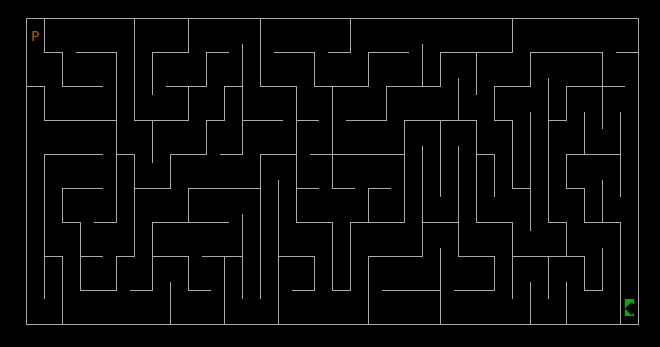
\includegraphics[width=1\textwidth]{rsrc/figure-title.png} \\
	\vspace{2em}
		{\large \@author} \\
		{\large Promotion ITII-P17} \\
		{\large\textbf{21 Mai 2018}}
	\vfill
	
	
\end{titlepage}
\makeatother

\tableofcontents

\chapter{Généralités}
\section{Introduction}

Ce document porte sur le projet informatique de deux étudiants de l’ITII PACA.

Le sujet proposé est la production d’un "jeu du labyrinthe".

Le projet a pour objectif de produire une application (un exécutable testé et
opérationnel) en situation de projet.

\section{Présentation  du projet}

Le sujet du projet est présenté en ligne dans le dossier "projet" de l'archive
suivante : \url{http://luc.hohwiller.online.fr/ITII2017/ITII2017.zip}.

\paragraph{}Il s’agit de réaliser un jeu de labyrinthe en 2 dimensions.

D’après \href{https://fr.wikipedia.org/wiki/Jeu_de_labyrinthe}{Wikipedia} :
\begin{quotation}
Le jeu de labyrinthe (en anglais, maze game) est un type de jeu vidéo dont le gameplay repose sur le motif du labyrinthe. L’objectif de jeu requiert de naviguer avec succès dans un labyrinthe, c’est-à-dire dans un décor sinueux, fait d’embranchements, d’impasses et de fausses pistes, destiné à perdre ou à ralentir le personnage. Il existe diverses variantes de ce type de jeux : la plus célèbre est sans doute celle incarnée par Pac-Man.
\end{quotation}
Ce travail est à réaliser par une équipe de 2 personnes en mode projet. Le code
à produire doit être du C ANSI. La présentation de l’application se fait sous
environnement Linux.

Le projet est géré en versions sous Github pour garantir sa sauvegarde.

\section{Présentation du document}

Ce document constitue le rapport présentant le travail effectué par le binôme de
MM. BATISTA Alan et GO Mathias de la promotion ITII-EII-P17.

\section{Plan du document}

Ce document est constitué comme suit :
\begin{itemize}
	\item \textbf{Chapitre 1 : Généralités} Introduction à ce document et au projet ;
	\item \textbf{Chapitre 2 : Synthèse} Compte-rendu succinct du projet ;
	\item \textbf{Chapitre 3 : Architecture} Organisation des sources et découpage fonctionnel ;
	\item \textbf{Chapitre 4 : Solutions techniques} Description de plusieurs des solutions techniques employées ;
	\item \textbf{Annexe A : Couverture des exigences} Matrice de couverture par rapport au cahier des charges ;
	\item \textbf{Annexe B : Contenu de la livraison} Description du contenu de la livraison ;
	\item \textbf{Annexe C : Manuel utilisateur} Explications sur l'utilisation du logiciel et description de son interface ;
	\item \textbf{Annexe D : Références} Liens vers les sources de différents codes exploités au cours de la production du projet.
\end{itemize}

% ##############################################################################
% ##############################################################################

\chapter{Synthèse}

\section{Avancement du projet}

A ce jour, le projet intègre les fonctionnalités suivantes :
\begin{itemize}
	\item Lecture de grilles à partir de fichiers ;
	\item Génération aléatoire de grilles ;
	\item Déplacement du joueur dans la grille ;
	\item Affichage du "fil d'Ariane" du joueur ;
	\item Affichage des murs "optimisé" ;
	\item Utilisation de menus de navigation.
\end{itemize}

Cependant, plusieurs fonctionnalités n'ont actuellement pas été implémentées :
\begin{itemize}
	\item Mode "Arcade" ;
	\item Menu de configuration du jeu.
\end{itemize}


\section{Répartition des tâches}

La répartition des tâches a été effectuée à partir de la liste de ces dernières.
Les étudiants ont choisi des tâches dans la liste du reste à faire au fur et à mesure de l'avancement du projet.

Cela a permis une répartition en corrélation avec l'évolution du niveau des étudiants :  
l’étudiant débutant en langage C a pu appréhender les notions importantes grâce à certaines fonctions spécifiques qu’il devra implanter. Notamment grâce aux explications de l’étudiant expérimenté, ce qui lui permettra petit à petit de pouvoir avancer plus efficacement.

\paragraph{}Ci-dessous le tableau récapitulatif de la répartition des tâches :

\paragraph{}
\begin{tabularx}{\linewidth}{|X|X|}
	\hline
	Tâche(s) & Etudiant \\
	\hline
	Gestion de la structure de données de la grille & GOM \\
	\hline
	Génération automatique de labyrinthe	& GOM	 \\
	\hline
	Création et récupération du labyrinthe dans un fichier txt & BAA \\
	\hline
	Création de la documentation & BAA \\
	\hline
	% Gestion des scores	& Mathias \\
	% \hline
	Gestion du déplacement du curseur &	BAA \\
	\hline
	Gestion de l'affichage & GOM \\
	\hline
\end{tabularx}








\chapter{Architecture}

\section{Architecture générale}

L'architecture du logiciel s'articule autour de plusieurs modules et sous-modules.

Nous avons identifié deux modules principaux : le module "ui" et le module "core", proposant respectivement les fonctionnalités d'affichage/gestion de l'interface utilisateur et des fonctionnalités relatives à la gestion des données.

Ci-après l'architecture des modules et sous-modules :
\begin{itemize}
	\item	\textbf{Module "core" :} Fonctions de traitement et de gestion des données :
	\begin{itemize}
		\item \textbf{core/grid} Gère les données de la grille de labyrinthe.
		\item \textbf{core/log} Permet de produire des fichiers de trace.
	\end{itemize}
	\item	\textbf{Module "UI" :} Gestion de l'affichage :
	\begin{itemize}
		\item \textbf{ui/common} Propose des fonctionnalités d'affichage diverses (defines, affichage de popups...).
		\item \textbf{ui/menus} Gère l'affichage des différents menus de l'application.
		\item \textbf{ui/play} Gère les différents modes de jeu.
	\end{itemize}
\end{itemize}

\section{Description des modules}
\subsection{Module "core"}
\subsubsection{Sous-module "grid"}

Ce sous-module permet de gérer le contenu de la grille du labyrinthe. Il gère un objet représentant le labyrinthe, sous la forme d'une matrice dont le contenu de chaque cellule est identifié par une valeur d'énuméré.
Le contenu de cet objet a été offusqué pour le reste du programme, ce qui permet de contrôler la manière dont le reste du programme accède aux données de la grille.

\paragraph{}
Les services proposés par ce module sont :
\begin{itemize}
	\item Création et destruction d'une grille ;
	\item Récupération d'informations à propos de la grille (nombre de lignes/colonnes) ;
	\item Lecture/écriture du contenu des cellules ;
	\item Fonctions de conversion du contenu d'une cellule vers un caractère et inversement ;
	\item Écriture du contenu d'une grille vers un fichier.
\end{itemize}


\subsubsection{Sous-module "log"}

Du fait que la console est utilisée pour l'affichage du programme, il n'est pas possible de l'utiliser pour afficher les traces du programme. Ainsi, pour permettre la production de traces de débogage, nous sommes passés par l'utilisation d'un module permettant d'écrire les traces dans un fichier texte.

Ce module propose également des macros de base permettant de rajouter des informations complémentaires dans les traces lors de leur écriture (nome de fichier, ligne, nom de la fonction...).

\paragraph{}
Les services proposés par ce module sont :
\begin{itemize}
	\item Ouverture et fermeture du fichier de traces ;
	\item Ecriture de traces.
\end{itemize}


\subsection{Module "UI"}
\subsubsection{Sous-module "common" (utils)}

Certains services d'affichage sont génériques et utilisés dans tous les modules (définition de styles d'affichage, affichage de popups...). Ces différents services sont regroupés dans ce module.

\paragraph{}
Les services proposés par ce module sont :
\begin{itemize}
	\item Définition des différents styles d'affichage pour \em{ncurses} et \em{CDK} ;
	\item Affichage centré d'un texte ;
	\item Affichage d'une popup bloquante ;
	\item Affichage d'une popup bloquante avec délai maximum ;
	\item Affichage d'une popup non-bloquante.
\end{itemize}


\subsubsection{Sous-module "menus"}

Ce module gère l'affichage et l'exécution des différents menus de l'application. Il est séparé en trois parties :

\begin{itemize}
	\item \textbf{ui\_menu} contient les parties communes relatives à la gestion d'un menu ;
	\item \textbf{ui\_menuPrincipal} contient la gestion du menu principal de l'application ;
	\item \textbf{ui\_menuPlay} contient la gestion des menus relatifs au lancement d'une partie de jeu.
\end{itemize}

L'affichage et la gestion des menus ayant recours à des algorithmes identiques peu importe le contenu du menu, plusieurs fonctions ont été utilisées dans "ui\_menu" pour encapsuler différents traitements comme la création/destruction de menus, d'items et l'affichage à l'écran d'un menu.

Les deux autres parties ("ui\_menuPrincipal" et "ui\_menuPlay") ne font qu'initialiser des structures de données représentant les items du menu, créer un menu, le redessiner et gérer les actions de l'opérateur en s'appuyant sur des services proposés par "ui\_menu".


\subsubsection{Sous-module "play"}

Ce module prend en charge la gestion des différents modes de jeu.

Chaque mode de jeu possède la même base de fonctionnement, la différence principale étant au niveau de la construction de la grille : le mode de jeu "selected" se base sur des grilles lues à partir de différent fichiers, alors que le mode "random" les génère aléatoirement.

\paragraph{}
Les services proposés par ce module sont :
\begin{itemize}
	\item Jouer à une grille créée aléatoirement ;
	\item Jouer à une grille lue à partir d'un fichier ;
	\item Services communs aux différents modes de jeu :
	\begin{itemize}
		\item Dessin d'une grille à l'écran ;
		\item Déplacement du joueur à partir de l'entrée clavier qu'effectue l'opérateur.
	\end{itemize}
\end{itemize}



% ##############################################################################
% ##############################################################################

\chapter{Solutions techniques}

\section{Fichier de données de grille}

Cette section décrit le format des "fichiers de grille".

Les grilles statiques du jeu sont stockées sous la forme de fichiers CSV (séparateur point-virgule).
Le choix de ce format a été guidé par sa simplicité d'utilisation et par le fait qu'il soit "humainement lisible".

Le tableau de données qu'un fichier représente est directement comparable à la représentation de la grille de jeu : chaque ligne du fichier représente une ligne de la grille ; la séparation entre les différentes cellules d'une même ligne est matérialisée par un point-virgule dans le fichier. Un caractère identifie le contenu de la cellule :
\begin{itemize}
	\item \textbf{E} représente une cellule vide sur laquelle le joueur peut se déplacer ;
	\item \textbf{W} représente une cellule "pleine" (mur) sur laquelle le joueur ne peut pas se déplacer ;
	\item \textbf{X} représente l'emplacement de la sortie du labyrinthe.
\end{itemize}

\newpage
\subsection{Exemple d'une grille simple}

Ci-après le contenu d'un fichier de grille et la représentation correspondante dans le jeu. Cette grille fait a une taille de 19 colonnes de largeur et 9 colonnes de hauteur.

\paragraph{Fichier de grille}
\begin{center}
	%\centering
	%\caption{Fichier de grille}
	\begin{BVerbatim}
	W;W;W;W;W;W;W;W;W;W;W;W;W;W;W;W;W;W;W
	W;E;E;E;W;E;E;E;E;E;E;E;E;E;W;E;E;E;W
	W;W;W;E;W;E;W;W;W;W;W;E;W;W;W;E;W;E;W
	W;E;E;E;W;E;E;E;E;E;W;E;E;E;E;E;W;E;W
	W;E;W;W;W;W;W;W;W;W;W;E;W;W;W;W;W;E;W
	W;E;W;E;E;E;W;E;E;E;W;E;E;E;E;E;W;E;W
	W;E;W;E;W;E;W;E;W;E;W;W;W;W;W;W;W;E;W
	W;E;E;E;W;E;E;E;W;E;E;E;E;E;E;E;E;X;W
	W;W;W;W;W;W;W;W;W;W;W;W;W;W;W;W;W;W;W
	\end{BVerbatim}
\end{center}

\paragraph{Représentation dans le jeu}
\begin{center}
	%\caption{Représentation dans le jeu}
	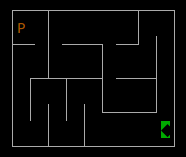
\includegraphics[width=0.5\textwidth]{rsrc/figure-grille_19x9.png}
\end{center}



\section{Gestion des données de la grille}

La gestion des données de la grille est effectuée dans le sous-module \mbox{"core/grid"}.

Le choix d'architecture a été porté par la volonté de garantir le bon usage de la structure de données correspondante. Cela nous a menés à créer une structure "privée" dont le contenu est masqué au reste du programme : seul le code contenu dans le fichier "grid.c" a accès au détail de cette structure.


\subsection{Structure de données}

La structure de données est composée de trois variables : Deux variables de type Entier identifiant le nombre de lignes et de colonnes de la matrice, et une variable de type pointeur sur énuméré "TEGridCellType" désignant l'espace mémoire alloué aux données de la grille.

Ci-après la déclaration de la structure tirée du fichier "grid.c" :
\begin{Verbatim}
struct  _SCoreGrid
{
	size_t  rowsCount;
	size_t  columsCount;
	
	TEGridCellType  *data;
};
\end{Verbatim}

Lors de la création d'une nouvelle grille via un appel à la fonction \verb|grid_create|, une allocation mémoire est effectuée pour une structure \verb|_SCoreGrid|. Ses membres \verb|rowsCount| et \verb|columsCount| sont initialisés à partir des paramètres passés à la fonction \verb|grid_create|. Ensuite, une allocation mémoire d'une taille de $\texttt{rowsCount} \times \texttt{columsCount} \times \texttt{taille de TEGridCellType}$ est effectuée et son adresse transmise au membre \verb|data| de la structure précédemment créée.


\subsection{Offuscation de la structure des données pour le reste du programme}

Pour faire en sorte que seul le module \mbox{core/grid} connaisse le contenu de la structure de données, nous avons procédé comme suit :

\begin{enumerate}
	\item \textbf{Déclaration de la structure de données \_SCoreGrid dans le fichier source du module.} Cela permet à l'ensemble des fonctions définies dans le fichier \verb|grid.c| d'avoir accès à la définition complète de cette structure.
	
	\item \textbf{Déclaration du type TCoreGrid en tant que pointeur sur \_SCoreGrid dans le header du module.} Ainsi, tout fichier ayant accès au fichier header \verb|grid.h| a accès à la déclaration de ce type et peut le manipuler.\\
	\textbf{Nota :} Cela fonctionne sans que la structure \verb|_SCoreGrid| soit déclarée dans le header car le nouveau type désigne un pointeur et non la structure en elle-même. Tous les pointeurs du système étant de la même taille, le compilateur n'a pas besoin d'avoir accès à la définition de la structure \verb|_SCoreGrid| pour allouer une variable de type \verb|TCoreGrid| et la manipuler.
	
	\item \textbf{Transmission d'une variable de type TCoreGrid lors de l'utilisation des fonctions du module \mbox{core/grid}.} Le reste du programme ne connaît que le type TCoreGrid ; cependant,  les fonctions du module ont accès à la fois à la définition du type \verb|TCoreGrid| et de la structure \verb|_SCoreGrid|. Elles peuvent ainsi manipuler le contenu du type \verb|TCoreGrid|.
\end{enumerate}

\paragraph{Extrait du fichier grid.c}
\paragraph{}
Ci-après la déclaration de la structure \verb|_SCoreGrid| et un exemple de fonction tirés du fichier \verb|grid.c| :
\begin{Verbatim}
#include "grid.h"

struct  _SCoreGrid
{
	size_t  rowsCount;
	size_t  columsCount;
	
	TEGridCellType  *data;
};

/* Exemple de fonction utilisant TCoreGrid */
size_t  grid_columnsCount(TCoreGrid argGrid)
{
	return  argGrid->columsCount;
}
\end{Verbatim}


\paragraph{Extrait du fichier grid.h}
\paragraph{}
Ci-après la déclaration du type \verb|TCoreGrid| et un exemple de fonction tirés du fichier \verb|grid.h| :
\begin{Verbatim}
typedef struct _SCoreGrid*  TCoreGrid;

/* Exemple de fonction utilisant TCoreGrid */
size_t  grid_columnsCount(TCoreGrid argGrid);
\end{Verbatim}


\subsection{Interaction avec les données}

L'interaction avec les données d'une grille se fait uniquement au travers des accesseurs déclarés dans le module.

Ci-après la liste des fonctions implémentés :
\begin{Verbatim}
/*
 * Fonctions de création/destruction de grille
 */
/** Fonction permettant de créer une grille. */
TCoreGrid   grid_create(size_t argRows, size_t argCols );

/** Fonction permettant de libérer proprement la mémoire allouée à une grille */
void        grid_destroy(TCoreGrid *argGridPtr );

/** Fonction permettant "d'imprimer" le contenu d'une grille dans un fichier */
void    grid_print(TCoreGrid argGrid , FILE* argFD);


/*
 * Fonctions retournant des informations à propos de la grille
 */
/* Retourne le nombre de colonnes (largeur) de la grille passée en argument */
size_t  grid_columnsCount(TCoreGrid argGrid);
 
/* Retourne le nombre de lignes (hauteur) de la grille passée en argument */
size_t  grid_rowsCount(TCoreGrid argGrid);


/*
 *  Fonctions de gestion des cellules
 */
/* Retourne le contenu d'une cellule */
TEGridCellType  grid_getCell( TCoreGrid argGrid,
                              size_t    argRow,
                              size_t    argCol );

/* Définit le contenu d'une cellule */
void            grid_setCell( TCoreGrid         argGrid,
                              size_t            argRow,
                              size_t            argCol,
                              TEGridCellType    argCellType );

\end{Verbatim}


%TODO \section{Gestion de l'affichage des murs}


% ##############################################################################
% ##############################################################################

\appendix % Permet de numéroter les chapitres suivant en tant que "Annexes".

%\chapter{Couverture des exigences}

%Ci-après la matrice de couverture des exigences. \\
%Voir page suivante.

%\begin{landscape}
%	mon beau tableau
%\end{landscape}


\chapter{Contenu de la livraison}

\section{Arborescence de l'archive}

La livraison contient les éléments suivants :
\dirtree{%
.1 (dossier racine).
	.2 docs/\DTcomment{Documents de la livraison}.
	.2 run/\DTcomment{Exécutable compilé et son environnement d'exécution}.
		.3 BAGOmaze\DTcomment{Exécutable}.
		.3 rsrc/\DTcomment{Dossier contenant les grilles statiques}.
	.2 sources/\DTcomment{Sources du logiciel}.
}

\section{Compilation des sources}

Le projet utilise \verb|qmake| et plusieurs autres dépendances.

Par commodité, un script \verb|install-dependecies-dev.sh| est disponible dans le dossier \verb|sources/BAGOmaze/| et permet d'installer les dépendances nécessaires à la majorité des systèmes Linux basés sur Debian comme Ubuntu.

Pour compiler les sources :
\begin{enumerate}
	\item Se rendre dans le dossier \verb|sources/BAGOmaze| ;
	\item Créer un sous-dossier \verb|build| ;
	\item Ouvrir un terminal dans le dossier \verb|build| ;
	\item Exécuter la commande \verb|qmake ..| ;
	\item Exécuter la commande \verb|make|
\end{enumerate}

L'exécutable est automatiquement déplacé dans le dossier \verb|BAGOmaze/out/app/|.


\chapter{Manuel utilisateur}

\section{Généralités}
\subsection{Introduction}

Cette section constitue le manuel utilisateur du projet BAGOmaze. Il explique comment naviguer dans les différents menus, configurer le jeu et se déplacer dans le labyrinthe.

\subsection{Arborescence des interfaces}
\dirtree{%
	.1 Main menu\DTcomment{Menu principal}.
		.2 Play\DTcomment{Menu de choix du mode de jeu}.
			.3 Arcade\DTcomment{Mode de jeu "time attack"}.
			.3 Choose level\DTcomment{Choix d'un niveau statique}.
				.4 Level 1.
				.4 Level 2.
				.4 Level 3.
				.4 Level 4.
				.4 Level 5.
			.3 Random\DTcomment{Génération aléatoire d'un niveau}.
		.2 Configure\DTcomment{Configuration de l'application}.
}



\section{Lancement du jeu}

Il est préférable de lancer le jeu à partir d'un terminal. Pour ce faire, ouvrir un terminal et se positionner dans le dossier contenant l'exécutable du jeu.

Pour lancer le jeu, exécuter la commande :
\begin{Verbatim}
	./BAGOmaze
\end{Verbatim}

Le jeu se lance en prenant la totalité de l'espace sur le terminal. Le menu principal de l'application apparaît.


\section{Menu principal}

\begin{center}
	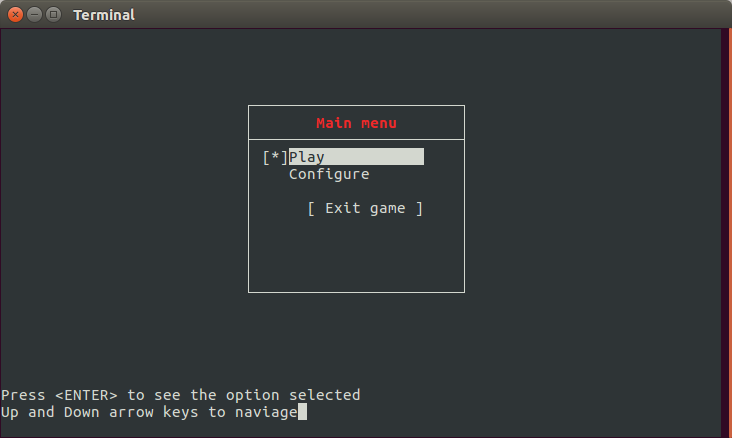
\includegraphics[width=0.75\textwidth]{annexe-manuel_utilisateur/rsrc/Main_Menu.png}
\end{center}

Le menu principal présente trois options :
\begin{itemize}
	\item \textbf{Play :} Permet d'accéder à l'écran de choix du mode de jeu.
	\item \textbf{Configure :} Permet d'accéder à l'écran de configuration du jeu.
	\item \textbf{Exit game :} Permet de quitter le jeu.
\end{itemize}

\paragraph{Nota :} L'écran de configuration n'est actuellement pas implémenté.

\paragraph{} L'opérateur peut naviguer entre les options en utilisant les touches directionnelles de son clavier pour mettre en surbrillance l'entrée du menu qu'il souhaite sélectionner. \\
Pour activer l'entrée du menu actuellement surlignée, l'opérateur doit presser la touche "Entrée" de son clavier.


\section{Menu "Play" - Choix du mode de jeu}

\begin{center}
	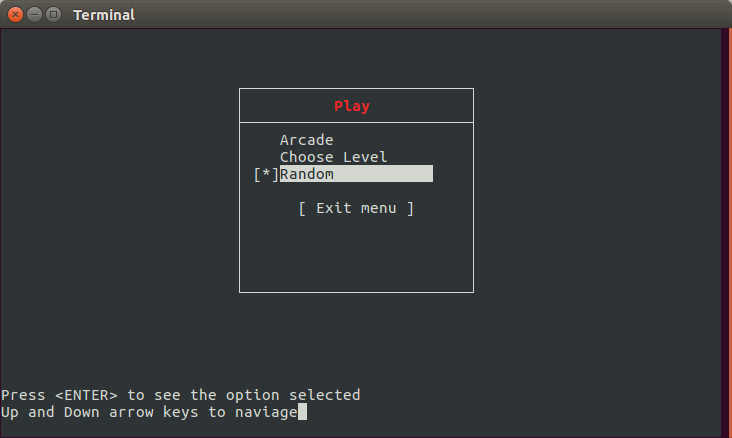
\includegraphics[width=0.75\textwidth]{annexe-manuel_utilisateur/rsrc/Menu_Play-random.png}
\end{center}

Dans ce menu, l'opérateur choisit le mode de jeu qu'il souhaite exploiter :
\begin{itemize}
	\item \textbf{Arcade :} Mode de jeu de type "time attack" dans lequel l'utilisateur doit résoudre des labyrinthes dans un temps imparti. Son score dépend du temps passé sur chaque labyrinthe et le nombre de déplacements qui lui ont été nécessaires pour sortir par rapport au nombre de déplacements nécessaires sur le chemin le plus court. Les dix meilleurs scores sont conservés en mémoire.
	\item \textbf{Choose level :} Mode de jeu dans lequel l'opérateur choisit entre cinq grilles prédéfinies chargées à partir d'un fichier.
	\item \textbf{Random :} Mode de jeu dans lequel une grille aléatoire est générée au lancement de la partie.
\end{itemize}

\paragraph{Nota :} Le mode de jeu "Arcade" n'est actuellement pas implémenté.

\paragraph{}La navigation dans ce menu est identique à celle du menu principal (touches directionnelles pour naviguer et touche "Entrée" pour valider).


\section{Menu "Choose level" - Choix d'une grille statique}

\begin{center}
	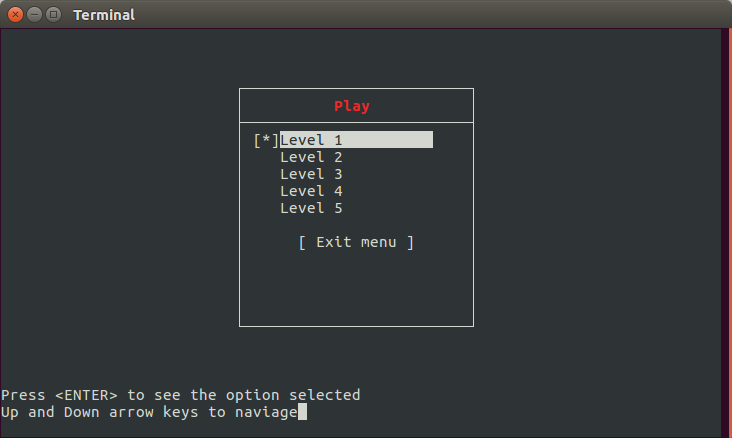
\includegraphics[width=0.75\textwidth]{annexe-manuel_utilisateur/rsrc/Menu_Play-grilles.png}
\end{center}

Ce menu apparaît lorsque l'opérateur sélectionne l'option \verb|"Choose level"| dans le menu \verb|"Play"|.

\paragraph{}L'opérateur peut choisir ici l'une des cinq grilles statiques inclues dans le jeu.

\paragraph{}La navigation dans ce menu est identique à celle du menu principal (touches directionnelles pour naviguer et touche "Entrée" pour valider).

\section{Gameplay}

Ci-après une capture d'écran d'un début de partie :
\begin{center}
	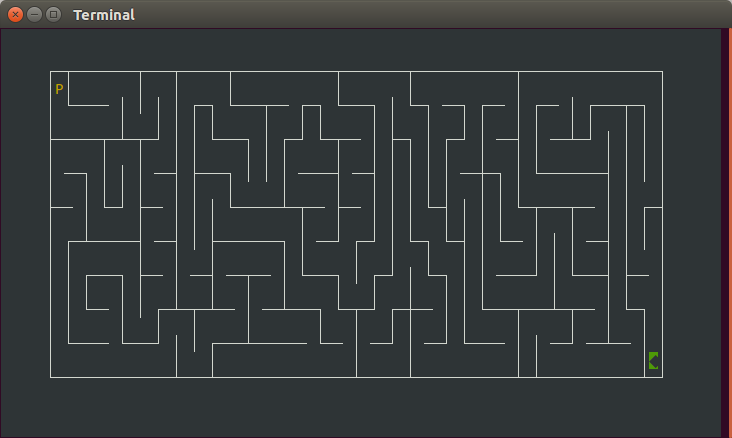
\includegraphics[width=0.75\textwidth]{annexe-manuel_utilisateur/rsrc/Labyrinthe-Debut.png}
\end{center}

La position du joueur est représentée par la lettre P clignotante, initialement située en haut à gauche de la grille.

La position de la sortie est représentée par le losange sur fond vert en bas à droite de l'écran.

Le but du jeu est pour le joueur de se déplacer dans le labyrinthe au moyen des touches directionnelles de son clavier dans le but d'atteindre la sortie.

Le chemin emprunté par le joueur ("fil d'Ariane") est représenté par de petits points au fur et à mesure de son avancée :
\begin{center}
	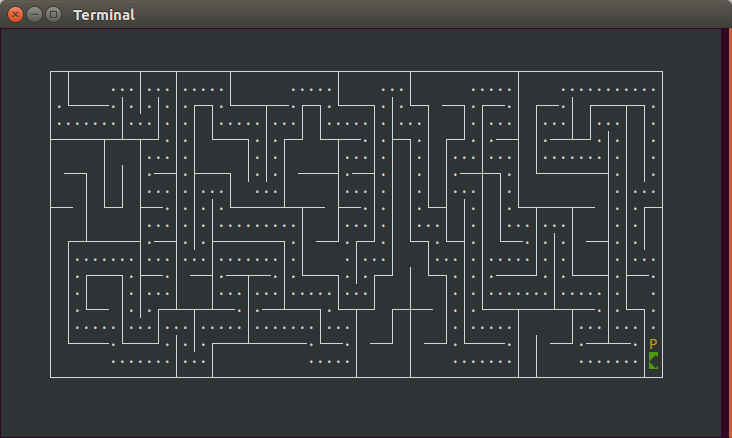
\includegraphics[width=0.75\textwidth]{annexe-manuel_utilisateur/rsrc/Labyrinthe-fin.png}
\end{center}

Une fois la partie terminée, une pop-up apparaît et le dernier menu utilisé ré-apparaît.


\chapter{Références}

\paragraph{Algorithme de génération aléatoire "DFS"}
\subparagraph{}Cet algorithme se trouve auprès de plusieurs sources sur Internet. Nous en avons récupéré une version que nous avons commenté pour en comprendre le fonctionnement, puis nous l'avons intégré à notre code source en l'adaptant pour qu'il s'interface avec notre code existant (module \mbox{core/grid} en particulier).

\subparagraph{}Cet algorithme possède certains atouts assez intéressant, en particulier le fait qu'il génère des labyrinthes sans "boucles" dans les chemins (pratique pour la gestion du "fil d'ariane" du joueur).

\subparagraph{Source :} \url{https://gist.github.com/kalmi/2953373}



\paragraph{Surcouche à ncurses : Librairie "CDK" (Curses Development Kit)}

\subparagraph{}Cette surcouche met à disposition du développeur des "widgets" encapsulant les fonctionnalités ncurses permettant de produire des interfaces graphiques plus facilement (fenêtres, dialogues, couleurs, styles,...).

\subparagraph{}Différents tutoriels et références existent sur Internet. Nous avons principalement exploité :
\begin{itemize}
	\item \url{http://invisible-island.net/cdk/}
	\item \url{https://connect.ed-diamond.com/GNU-Linux-Magazine/GLMF-107/ncurses-facile-avec-CDK}
\end{itemize}


\end{document}